\documentclass[utf8, a4paper]{beamer}

\usepackage[english]{babel}
\usepackage[T1]{fontenc}

\usepackage{amsmath, amsfonts, graphicx}
\usepackage{bibunits, tikz}

\usetheme{progressbar}

\setbeamersize{text margin left=1em, text margin right=1em}

\title[PCA]{Principal Component Analysis:\\dalla teoria alla pratica}

\author[Marco Buracchi]{Marco Buracchi}

\date{\today}

\institute{Università degli studi di Firenze}

\graphicspath{{img/}}

\begin{document}

\maketitle

\begin{frame}{Sommario}

  \tableofcontents

\end{frame}

\section{Principal Component Analysis}

	\begin{frame}{PCA}
		Intro
	\end{frame}

	\subsection{Cosa fa?}
		\begin{frame}{PCA}
			Cosa fa?
		\end{frame}
		
	\subsection{Come funziona?}
		\begin{frame}{PCA}
			Come funziona?
		\end{frame}
	
\section{Implementazione Python}

	\begin{frame}{Implementazione}
		Come è stato implementato
	\end{frame}

	\subsection{PANDAS}
		\begin{frame}{PANDAS}
			PANDAS
		\end{frame}
	
	\subsection{Implementazione}
		\begin{frame}{Implementazione}
			\begin{itemize}
				\item Preparazione dataset
				\item Calcolo autolavori/vettori
				\item Selezione delle componeni
				\item Matrice di proiezione
				\item Proiezione
			\end{itemize}
		\end{frame}

\section{Caso di studio}
	\begin{frame}{Caso di studio}
		Caso di studio
	\end{frame}

	\subsection{Attacchi}
		\begin{frame}{Attacco SMURF}
			\begin{figure}
				\begin{center}
					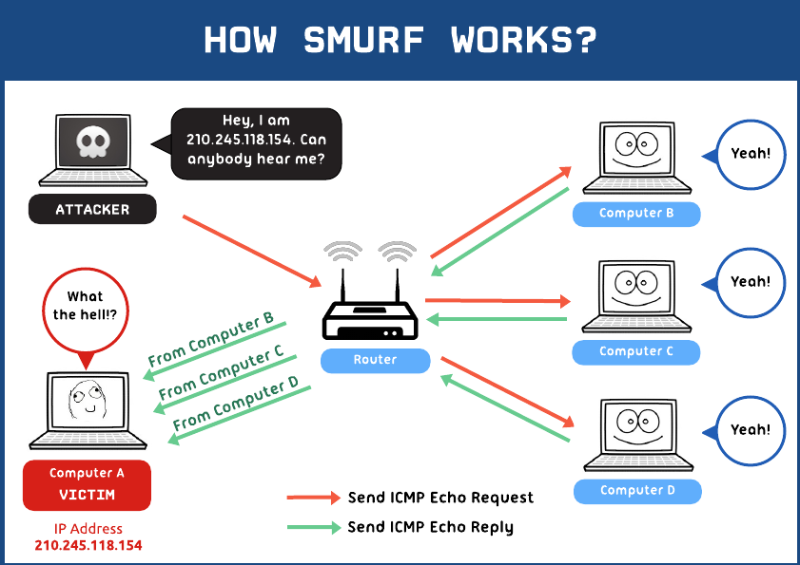
\includegraphics[width=.75\textwidth]{smurf}
				\end{center}
			\end{figure}
		\end{frame}
		\begin{frame}{Attacco Neptune}
			\begin{figure}
				\begin{center}
					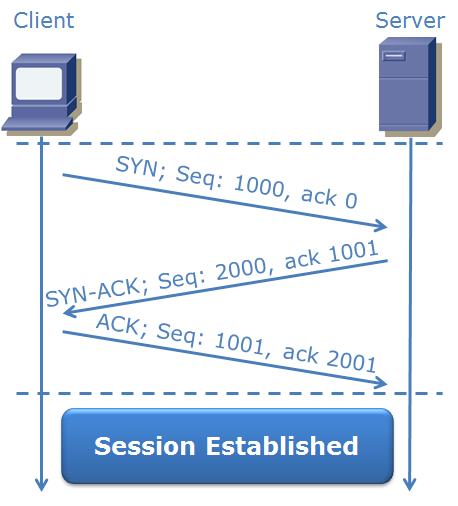
\includegraphics[width=.5\textwidth]{3wayh}
				\end{center}
			\end{figure}
		\end{frame}
		
		\begin{frame}{Attacchi Network Probe}
			NP
		\end{frame}
	
	\subsection{Analisi}
		\begin{frame}{Analisi}
			Preprocessing
		\end{frame}
	
	\subsection{Risultati}
		\begin{frame}{Rilevazione}
			Rilevazione
		\end{frame}
	
\section*{Bibliografia}	
	\begin{frame}{Bibliografia}
		\nocite{anderson2003introduction,mardia1979multivariate,pandasManual,pandasSite,Labib2006}
		\bibliography{bibliografia}
		\bibliographystyle{unsrt}
	\end{frame}

\end{document}
